%\chapter{Discrete Choice Modeling Perspective on MATSim \who{Flötteröd}}
\chapter{Choice Models in MATSim}
\label{ch:discretechoice}
% ##################################################################################################################

\hfill \textbf{Author:} Gunnar Flötteröd, Benjamin Kickhöfer

%\gunnar{Equation underlying the ``title figure'' has changed.} \ah{corrected}

\begin{center} 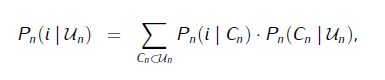
\includegraphics[width=0.5\textwidth, angle=0]{understanding/figures/dc.png} \end{center}

% ##################################################################################################################
This chapter (i) attempts to reconcile \gls{matsim}'s mechanisms of plan
{}``mutation'', {}``selection'' and {}``execution'', borrowed from evolutionary computation, with a 
%mainstream
discrete choice perspective, and (ii) and sketches a possible solution to the
plan choice set generation problem. Parts of the following text are taken from \citet[][Section~2.3]{Kickhoefer_PhDThesis_2014}.

Discrete choice theory goes back to work by \citet{Luce1965PreferenceUtility} and 
\citet{McFadden1975DiscreteChoiceModel}. Two standard textbooks in this area are by
\citet{BenAkivaLerman_1985} and by \citet{Train_2003}. The theory is mainly used 
to describe individual choices among \emph{mutually exclusive} alternatives. 
Discrete choice models typically do not perfectly predict individual choices.
\citet{Luce1965PreferenceUtility} distinguish between two possible interpretations of this phenomenon:
(1) People choose randomly among their alternatives, rendering their behavior inherently unpredictable.
(2) The choice only \emph{appears} to be random since the modeler does not include all relevant 
decision variables in the model. 
%However, 
Both perspectives lead to the same result, namely the %adaptation
introduction
of probabilistic choice models.

Let $\mathcal{U}_n$ be the universal set of all plans that may ever be considered
by agent $n$, and denote by $C_{n}$ the concrete plan choice set
of that agent. The choice set independent probability that agent $n$
selects plan $i$ for execution can then be written as
\begin{eqnarray}
P_{n}(i\mid \mathcal{U}_n) & = & \sum_{C_{n}\subset \mathcal{U}_n}P_{n}(i\mid C_{n})\cdot P_{n}(C_{n}\mid \mathcal{U}_n),
\label{eq:unconditional-choice-proba}
\end{eqnarray}
which means the following. Selecting a plan requires a plan choice
set. The term $P_{n}(C_{n}\mid \mathcal{U}_n)$ represents the probability that
this concrete choice set is $C_{n}$, which must be a subset of $\mathcal{U}_n$.
Technically, the plan \emph{innovation} modules draw from this distribution.
The term $P_{n}(i\mid C_{n})$ represents the probability that agent
$n$ selects plan $i$ given that its concrete choice set is $C_{n}$.
Technically, the plan \emph{selection} modules draw from this distribution.
The product of these terms hence represents the probability that both
the choice set $C_{n}$ is available and that plan $i$ is chosen out
of that set. The probability of selecting plan $i$ independently
of the concrete choice set then results from adding the probabilities
of selecting it in the presence of all possible choice sets $C_{n}\subset \mathcal{U}_n$.

One observes in \MyEqRef{eq:unconditional-choice-proba} that the
behavior of an agent depends on both the choice model and the way
in which the choice set is generated, both of which are addressed
in the following.

% ##################################################################################################################
\section{\label{sec:Evaluating-choice-models}Evaluating Choice Models in
a Simulated Environment}

The discussion provided in this section focuses on the choice distribution
$P_{n}(i\mid C_{n})$ for given choice sets. In \gls{matsim}, a plan is
evaluated in terms of its score, and plan selection is based on the
score as the sole property of the plan. This is only a technical specification;
the scoring and selection protocols are responsible of representing
adequate perceptional and behavioral mechanisms. The notions of {}``choice''
and {}``selection'' are subsequently used interchangeably (\cf Section~\ref{sec:selectors}).

The usual selection protocol of \gls{matsim} resembles a \gls{mnl}
choice model. Letting $S_{ni}$ be the score of plan $i$ of agent
$n$, one has
\begin{eqnarray}
P_{n}(i\mid C_{n}) & = & \frac{e^{\mu S_{ni}}}{\sum_{j\in C_{n}}e^{\mu S_{nj}}}\label{eq:ExpBetaPlanSelector}
\end{eqnarray}
with $\mu$ controlling the preference for higher scores.
It is set to one in the remainder of this section. 

\subsection{Case 1: Score is or converges towards a deterministic value}

Only if the score
of a plan was a deterministic number representing an expected value, 
then Equation~(\ref{eq:ExpBetaPlanSelector}) would constitute a plain \gls{mnl} choice model with $\mu$ taking the role
of a scale parameter \citep[see, e.g.,][p.45]{Train_2003}. 
Such behavior 
can be approximated in \acrshort{matsim} by the following configuration settings:
\begin{itemize}
\styleItemize
\item A fixed choice set $C_n$ is eventually obtained by setting the configuration option \verb$fractionOfIterationsToDisableInnovation$ below one,  
meaning that for the remaining fraction of iterations beyond the configured value, innovation will be switched off.
%% \ie the choice sets will remain fixed from then on;
\item Score convergence to its expectation value can be achieved by setting the configuration option \verb$fractionOfIterationsToStartScoreMSA$ below one, 
meaning that for the remaining fraction of iterations scores will be averaged according to the \acrfull{msa}.
\end{itemize}
%
%% \benjamin{Ich verstehe nur bedingt, warum diese 2 Punkte zu einem ``plain MNL choice model'' führen sollen; denn die choice set generation (welche in diesem Teil des Kapitels gar nicht behandelt wird), kommt hier auf einmal doch vor...diese 2 Punkte beziehen sich doch eher auf Eq.~\ref{eq:unconditional-choice-proba}, oder?}

\subsection{Case 2: More general}

Without this particular configuration, things are somewhat more complicated.

Assume that the attribute vector $\mathbf{x}_{ni}$ of the alternatives in \MyEqRef{eq:ExpBetaPlanSelector}
is defined through (a transformation of) the network conditions observed
during the last iteration(s). Assume further that the score is a linear
function of these attributes:
\begin{eqnarray}
S_{ni} & = & \boldsymbol{\beta}^{T}\mathbf{x}_{ni}\\
 & = & \boldsymbol{\beta}^{T}(\text{E}\{\mathbf{x}_{ni}\}+\boldsymbol{\eta}_{ni})\label{eq:score}
\end{eqnarray}
where $\boldsymbol{\beta}$ is a coefficient vector, superscript $T$ denotes the transpose,
and $\boldsymbol{\eta}_{ni}$ is a zero mean random vector. 
In the general case of $S_{ni}$ being a random
variable and not just an expected value, one obtains a mixture-of-logit
model with the choice distribution
\begin{eqnarray}
P_{n}(i\mid C_{n}) & = & 
\int\frac{\exp\left(\boldsymbol{\beta}^{T}\text{E}\{\mathbf{x}_{ni}\}+\boldsymbol{\beta}^{T}\boldsymbol{\eta}_{ni}\right)}
{\sum_{j\in C_{n}}\exp\left(\boldsymbol{\beta}^{T}\text{E}\{\mathbf{x}_{nj}\}+\boldsymbol{\beta}^{T}\boldsymbol{\eta}_{nj}\right)}
p(\boldsymbol{\eta}_{n})d\boldsymbol{\eta}_{n}\label{eq:mixture-of-logit}
\end{eqnarray}
where $p(\boldsymbol{\eta}_{n})$ is the probability density function of 
$\boldsymbol{\eta}_{n}=(\boldsymbol{\eta}_{ni})_i$ \kai{@Gunnar: I added 2nd index $i$, pls chk}, \ie the joint probability
density function of the random disturbances of all alternatives of individual $n$
\citep{Train_2003}. This formulation comprises most if not all \gls{matsim}
configurations currently used. It represents the \lstinline{ExpBetaPlanSelector}
and the equivalent \lstinline{ExpBetaPlanChanger}. It also comprises
the \lstinline{BestPlanSelector} because that is equivalent to the \lstinline{ExpBetaPlanSelector}
with a very large (infinite) $\mu$. Arbitrary score averaging schemes
are also included; this only leads to different instances of $p(\boldsymbol{\eta}_{n})$.

Mainstream applications of mixture-of-logit models attempt to combine
the tractability of closed-form logit models with the flexibility of
simulating arbitrary $p(\boldsymbol{\eta}_n)$ distributions.
The distribution of $\boldsymbol{\eta}_n$ is often as simple as a multivariate normal
because this already allows to introduce rich correlation structures
into the underlying random utilities. In \gls{matsim}, however, the simulated
error term $\boldsymbol{\eta}_n$ is extremely complicated. Revisiting \MyEqRef{eq:score},
it defines the variability of the score that results from the fact
that the simulated network conditions are stochastic. The distribution
from which these network conditions are drawn is defined implicitly
through the mobility simulation. It is not available in closed form;
one can only draw from it.

Additional complexity results from the simulated network conditions
being in turn the consequence of simulated travel behavior that is
again defined through \MyEqRef{eq:mixture-of-logit}. 
%% This circular
%% dependency is natural, given that \gls{matsim} is mainly a transport planning
%% model (see Chapter~\ref{ch:montecarlo}).
%% %
%% \benjamin{Dies verstehe ich nicht, klingt ein wenig abwertend. Wieso muss das in einer Transportsimulation so sein? Wie wäre es denn wenn MATSim eine Börsensimulation wäre? Ähnlich oder? Ansonsten sehr schön formuliert, man versteht, dass wir auch nicht wissen, was alles in $\boldsymbol{\eta}_n$ drinsteckt :)}
%% %
%% Indeed, 
Just as a representation
of the mutual demand/supply dependency is essential in transport planning,
the circular definition of the $\boldsymbol{\eta}_n$ terms adds realism to \gls{matsim}:
\begin{enumerate}
\item Assume one could somehow make the simulated network conditions more
realistic. The result would be a more realistic distribution $p(\boldsymbol{\eta}_n)$
of the simulated error terms.
\item All else equal, increasing the realism of $p(\boldsymbol{\eta}_n)$ in \MyEqRef{eq:mixture-of-logit}
would also increase the realism of the resulting choice distributions.
\item This in turn would lead to the selection of more realistic travel
plans, with the consequence that their execution would result in even
more realistic network conditions.
\end{enumerate}
However, this positive feedback only applies to the extent to which
the random error terms of the postulated behavioral model are indeed
outputs of the mobility simulation. Simulated travel time (variability)
is such a case. Unobserved preferences of the decision maker, however,
are not an output of the mobility simulation and hence need to be
captured otherwise. 
%% (The extreme case of a choice distribution that
%% results from combining a stochastic mobility simulation with a best-response
%% plan selection hence constitutes only a limited, so to say {}``mechanical''
%% perspective on travel behavior.)


\subsection{Illustrative example of how this could be used}

%% %% \subsection{\label{sec:convergence}???Randomness and Self-Consistent State???}
%% %
%% \benjamin{Alternativer Titel: ``Convergence under Stochastic Network Conditions''}
%% %
%% \benjamin{Alternativer Titel: ``Stochastic Network Conditions and Stationary Distribution''}
%
How to insert the randomness of the simulated network conditions into
$\boldsymbol{\eta}_n$ is a delicate problem.
%
\benjamin{Führen wir Randomness in $\boldsymbol{\eta}_n$ ein oder existiert sie nicht einfach aufgrund der Simulation, des Verhaltensmodells etc.? Vielleicht umformulieren?} 
%
The notion of {}``learning'' again
enters the picture, and again it is not particularly helpful, cf.~Chapter~\ref{ch:montecarlo}: If the simulation iterations really represented
simulated days, then a model of real human learning would be needed in
order to combine a sequence of past network conditions into an instantaneous
$\boldsymbol{\eta}_n$ realization. Without a sound instance of such a learning model,
a behavioral justification of \MyEqRef{eq:mixture-of-logit} cannot
be given.

However, another perspective on this problem is possible, continuing
the arguments of Chapter~\ref{ch:montecarlo}. It is argued there that one can consider
the sole purpose of \gls{matsim}'s iterative mechanism to attain a realistic
stationary distribution. If so, then the sole purpose of the simulated
$\boldsymbol{\eta}_n$s is to yield a realistic stationary choice distribution. To
illustrate this perspective, consider the following moving-average score
updating rule:
\begin{eqnarray}
\bar{S}_{ni}^{k+1} & = & \begin{cases}
\alpha S_{ni}^{k} + (1 - \alpha)\bar{S}_{ni}^{k} & \text{if }n\text{ chose plan }i\\
\bar{S}_{ni}^{k} & \text{otherwise}
\end{cases}
\end{eqnarray}
where $\bar{S}^{k}$ is the filtered score of iteration $k$ and $S^{k}$
is the concrete score observed in that iteration. The learning rate $\alpha$
controls how strongly the filtered score is smoothed out, and hence
it controls the variability of $\boldsymbol{\eta}_n$. \gls{matsim} enables this mechanism
through the \lstinline{learningRate} parameter.
%
\benjamin{Was ist denn dann die praktische Empfehlung für $\alpha$? Welcher Wert ist sinnvoll?}

Assuming for simplicity that upon convergence the unfiltered stationary score
$S_{ni}^{\infty}$ fluctuates independently from iteration to
iteration around its expected value, one can derive the following 
(as demonstrated in the appendix to this chapter):
\begin{eqnarray}
\text{E}\{\bar{S}_{ni}^{\infty}\} & = & \text{E}\{S_{ni}^{\infty}\}\\
\text{VAR}\{\bar{S}_{ni}^{\infty}\} & = & \frac{\alpha}{2-\alpha}\text{VAR}\{S_{ni}^{\infty}\}.
\end{eqnarray}
$\bar{S}$ is unbiased with respect to the underlying score process
and its variance is in the interval from zero to $\text{VAR}\{S\}$,
depending on the chosen $\alpha$. There is no need to justify this
through a learning process. One merely has constructed a parametrization
of the distribution $p(\boldsymbol{\eta}_n)$. In the resulting
mixture model \MyEqRef{eq:mixture-of-logit}, $\alpha$ should be
estimated from real data, just as any other parameter of that model.
%
\benjamin{Wenn man das schätzen soll, frage ich mich wie das praktisch geht. Was für Daten braucht man? Außerdem sehe ich gar kein $\alpha$ in Eq.~\ref{eq:mixture-of-logit}; man müsste dann ggf. erklären, wo es sich dort versteckt. Denn ich sehe, dass es mehrere $\beta$ gibt, aber...}

\kai{Hier stand ein Abschnitt über ``frozen randomness''.  Ich habe das jetzt wg.\ Nichtkonvergenz der Diskussion nach ``research avenues'' befördert.  Hoffe mal, dass wir uns dort dann über das wording einigen können, sonst haben wir ein Problem, wenn wir noch nicht einmal die Forschungsfrage formulieren können. :--)}

%% \subsection{\label{sec:stochasticity-and-repeated-choices}Stochasticity and Repeated Choices -- ???Sources of Stochasticity???}
%% %
%% \gunnar{Der Fokus dieses Abschnittes sollte auf der day-to-day correlation der epsilons liegen.
%% Benjamin, willst Du Dich einmal daran versuchen, das hier einzubauen?}
%% %
%% \gunnar{Wenn man es hier l\"asst, sollte zumindest der (terminologische) Zusammenhang zur Mainstream-Literatur
%% sichergestellt werden. Es gab da mal eine Diskussion \"uber ``quenched/frozen randomness'' vs. ``random effect model'',
%% die hatte irgendwie ein Ende gefunden, aber ich weiss nicht mehr, was der Konsens war.}


%% %% \gunnar{Zudem frage ich mich, ob es hier auch einen Bezug zu ``Sobol''- oder ``Niederreiter''-Sequenzen gibt, 
%% %% von welchen mir gesagt wurde, dass sie irgendwie random number sequences anhand eines niedrigdimensionalen 
%% %% ``Startvektors'' initialisieren. Solche Sequenzen kommen offenbar bei der Sch\"atzung simulationsbasierter choice 
%% %% models zum Einsatz kommen.

%% %% Ich habe mir das aber selber noch nicht angeschaut.
%% %% }

%% %% \kai{Für mich hört sich das verwandt an zu Halting-Sequenzen o.ä.  Das sind Sequenzen, die insbesondere vieldimensionale Räume gleichmäßiger überdecken als reine Zufallszahlen, aber doch kein periodisches Gitter bilden.  Chandra Bhat benutzt so etwas auch.  Man könnte einen Zusammenhang mit dem Thema hier konstruieren, aber das scheint mir nicht sofort naheliegend und damit bestenfalls (wenn jemand es ausformulieren will) research avenues.}

%% \benjamin{Ja, habe ich versucht. Allerdings finde ich die Ankopplung als eigene (Main)Section eher unglücklich. Habe mal einen Vorschlag gemacht, wie man Teile von deinem Text vorher in eine Subsection schieben könnte, und dies hier dann die zweite Subsection von ``Evaluating Choice Models...'' werden könnte.}

%% %% \begin{oframed}

%% %% \citet{McFadden1975DiscreteChoiceModel} built his \gls{rum} by introducing a \emph{random component} into the utility formulation:
%% %% %
%% %% \begin{equation}
%% %% U_i = V_i + \varepsilon_i \ ,
%% %% \end{equation}
%% %% %
%% %% where $U_i$ is the utility of alternative $i$, which is \emph{perceived} by the individual; $V_i$ is the observed or systematic part of utility%
%% %% %
%% %% %described by the utility function (see Equation~\ref{XXX})%
%% %% %
%% %% %\benjamin{Some reference to the utility function of a plan}
%% %% %%
%% %% %\benjamin{I would strongly recommend to use $V_p$ instead of $U_p$ for the utility of a plan even though this is not entirely true, since some of the $\epsilon$ is already captured by the simulation noise that Gunnar called $\eta$...In consequence, the score is NOT equal to $V_p$, right?}
%% %% %%
%% %% %\benjamin{Maybe remove the \acrshort{matsim} reference here completely, and deal with the issue above in the \acrshort{matsim} section below?}
%% %% %%
%% %% %\kai{intuition to remove reference to matsim here.}
%% %% %%
%% %% %\benjamin{Agreed. Removed it, and copied my comment further down.}
%% %% %
%% %% ; and $\varepsilon_i$ is a random component of utility.
%% %% %
%% %% As a result, the random component allows to chose options which do not have the highest utility with respect to $V_i$.
%% %% %% for choices that are -- according to the systematic parts of utility calculated by the utility functions -- \emph{irrational}. In consequence, there is a \emph{probability} to select the option with the highest $V_p$, as well as (lower) probabilities to select the other options with lower $V_p$. 
%% %% %
%% %% % Habe obiges mal rausgestrichen, weil man m.E. Annahmen über eps (meiner Intuition nach: Mittelwert=0) machen muss, damit die Aussage wirklich stimmt.  kai, oct'14

%% %% Assuming that all $\varepsilon_i$ are independent and identically distributed (i.i.d.)\ following a Gumbel distribution, this leads to an \gls{mnl} model with the choice probability $P_i$ for alternative $i$:
%% %% %
%% %% \begin{equation}
%% %% P_{i} = \frac{e^{\mu \cdot V_i}}{\sum_{j=1}^{J} e^{\mu \cdot V_{j}}} \ ,
%% %% \label{eq:ch:economicEval:logit}
%% %% \end{equation}
%% %% %
%% %% %% \kai{Notation für die Summe im Nenner habe ich so noch nie gesehen.  chk}
%% %% %% %
%% %% %% \benjamin{Habe es mal anders notiert. Ben-Akiva schreibt $\sum_{j \in C_n}$, wobei $C_n$ das choice set des Individuums ist. Allerdings bekommen wir mit $j$ als Index an anderen Stellen Probleme...}
%% %% %
%% %% where $J$ is the total number of alternatives in the choice set, and $\mu$ is related to the variance of the random component.%

%% %% From the modeler's perspective, $\mu$ describes how rational (with respect to the model) decision makers behave, given a difference in the systematic part between utilities of alternatives. To give an example on the influence of $\mu$ on the choice probabilities of $J=2$ alternatives $a$ and $b$ with $V_b > V_a$: following Equation~\ref{eq:ch:economicEval:logit}, the corresponding choice probabilities are given by
%% %% %
%% %% \[
%% %% P_a = \frac{1}{1 + e^{\mu(V_b - V_a)}} \qquad P_b = \frac{1}{1 + e^{\mu(V_a - V_b)}} \qquad .
%% %% \]

%% %% %
%% %% As one can see, the choice probabilities only depend on the difference between the systematic parts of utility $V_a - V_b$,%
%% %% %
%% %% \footnote{
%% %% %
%% %% It can therefore be argued that with the use of Discrete Choice Theory, one has already left the ground of an ordinal scale of utility, since the difference in utility influences the choice probabilities.
%% %% %
%% %% }
%% %% %
%% %% and on the parameter $\mu$.
%% %% %
%% %% For $\mu \to 0$, this results in a completely random choice behavior and choice probabilities of $P_a = P_b = \frac{1}{2}$.
%% %% %
%% %% For $\mu \to \infty$, this results in a completely ``rational'' behavior and choice probabilities of $P_a = 0$ and $P_b = 1$.
%% %% %
%% %% The first case corresponds to a very large variance, the latter to a very small variance of the difference between the random components $\varepsilon_b - \varepsilon_a$.


%% As pointed out at the beginning of this section, the score of a particular plan of a particular individual\textemdash as a result of stochastic network conditions\textemdash varies over iterations. 

%% An issue is that the randomness that is explicitly contained in MATSim needs to be consistent with the discrete choice model.
%% %% \footnote{
%% %% %
%% %% \benjamin{Some pointer to Gunnar's chapter where it is discussed under what conditions $S_{n,i} = V_{n,i}$ or $S_{n,i} = U_{n,i}$ or something completely else.}
%% %% %
%% %% }
%% %
%% For example, the propensity to use public transit might depend on the distance to the next transit stop, or how well that stop connects to the destination to which the person is traveling.  \acrshort{matsim} will pick up such effects explicitly.  Only a choice model which considers the same attributes will be consistent; otherwise, some of the above effects will be considered as random from the point of view of the analyst and thus be moved into the $\varepsilon_i$, and subsequently into the scale parameter $\mu$.

%% The interpretation in Section~\ref{ch:economicEval:describingBehavior:discreteChoice:quenchedVsAnnealed} assumes that each \acrshort{matsim} agent performs repeated random draws according to its choice set and its choice model. 
%% %
%% In other words:
%% %
%% \begin{itemize}\styleItemize
%% \item It is assumed that the scores $S_{n,i}$ have converged and correspond to the systematic parts of utility $V_{n,i}$. In consequence, also the choice probabilities $P_{n,i}$ have converged.
%% %
%% \item However, making repeated random draws from these probabilities effectively \emph{parametrizes} the effect of randomly re-drawing the $\varepsilon_{n,i}$, and then taking the option $i$ where $U_{n,i} = V_{n,i} + \varepsilon_{n,i}$ is maximal. That is, the alternative with the highest utility might vary.
%% \end{itemize}
%% %

%% Alternatively, the approach presented in Chapter~\ref{ch:destinationchoice} ``freezing'' the epsilons directly into the plans can be applied.  
%% In this interpretation, each plan $i$ obtains a fixed $\varepsilon_{n,i}$ at construction, which only changes when the plan changes. 
%% In consequence, once the choice set becomes fixed, also each plan's $\varepsilon_{n,i}$ becomes fixed, and the choice model should then deterministically select the plan with the highest score \emph{including the plan's $\varepsilon_{n,i}$}.
%% That is, the score $S_{n,i}$ would be directly interpreted as the total utility $U_{n,i}$.
%% Such an approach can currently not be applied out-of-the-box for \acrshort{matsim} for other choice dimensions than destination choice (Chapter~\ref{ch:destinationchoice}).
%% To date, it needs to be programmed explicitly in \gls{java}, research to extend this to all choice dimensions is underway (Section~\ref{sec:future-frozen-randomness}). 

%% %% \end{oframed}



% ##################################################################################################################
\section{Evolution of Choice Sets in a Simulated
Environment}
\label{sec:Evolution-of-choice}

The choice set of agents can in principle be pre-computed and then be fed into the \acrshort{matsim} simulation. However, this would need to be done for every system state (\eg before and after a policy change).
%
Alternatively, \acrshort{matsim} can generate choice sets of agents within the iterative loop (Section~\ref{sec:inbrief}).
%
%\benjamin{Some reference to the loop.}%
%


\subsection{Issues}
\label{sec:Evolution-of-choice:issues}

\kai{Mit Benjamin besprochene Tendenz, diese section hier wieder rauszunehmen und sie woanders unterzubringen.  Ansonsten passt das u.E.\ nicht gut zusammen: Die issues machen doch sehr deutliche Aussagen über eine Reihe von Herausforderungen.  Die Theorie ist hingegen \emph{ein} (wenn auch wichtiger) Lösungsansatz; andere Ansätze, die stärker heuristisch ABER dafür bereits implementiert sind, gibt es ja auch.  --- Ich überlasse das Verschieben aber mal Benjamin.}

At the time of writing, there exist three methodological issues when generating on-the-fly choice sets with \acrshort{matsim}:
%
\begin{enumerate}\styleEnumerate
\item \textbf{Choice set incomplete}: The maximum number of plans $J$ in the choice set of every agent is limited by computer memory constraints. That is, the choice set for the decision making is unlikely to be complete.
%
\item \textbf{Plans correlation from innovation}: Plans might be correlated. This is very likely if they are modified or replaced by best-response re-planning modules (\eg the route choice module), since they have a tendency to always generate the same answer. Yet also random mutations in general result in correlated plans, since the concept of a mutation in fact implies an only small change away from the parent.  This violates the required IIA (Independence from Irrelevant Alternatives) 
% _from_ !!
property of the choice set that is needed for an \gls{mnl} 
% _an_ eMeNel !!
model.\footnote{%
%
A possible approach to increase the diversity in route choice is investigated by \citet{NagelKickhoeferJoubert2014HeterogeneousVoTsPROCEDIA}.
%
} Also see Section~\ref{sec:heterogeneity-in-plans-generation}.

\item \textbf{Plans correlation from plans removal}: The current \acrshort{matsim} implementation has a tendency to keep similar, \ie  correlated, plans when the number of plans has grown beyond $J$.  The reason for this is that the current plans remover removes the plan with the lowest score, which typically also is the one most different from the other plans.  As a result, typically only very similar plans with very similar scores remain in the choice set.\footnote{%
%
A possible approach to maintain diversity in plans removal would be to give penalties to the scores of plans that are similar to other plans.  This penalty could be taken directly from approaches such as the path size logit \citep{DaganzoSheffi_TransScience_1977,FrejingerBierlaire_TransResB_2007}.  For early attempts within \acrshort{matsim} see \cite{Grether_PhDThesis_2014} (Chapter~6) and \cite{NeumannEtAlPassengerArrivalPatterns}.
%
} Also see Section~\ref{sec:heterogeneity-in-plans-removal}.
%
\end{enumerate}
%
These three issues might lead to biased behavior, which also has consequences for economic evaluation (see Chapter~\ref{ch:economicEval}).

\subsection{Possible Solution}
\label{sec:Evolution-of-choice:solution}
\benjamin{Das ist ein harter Bruch an dieser Stelle. M.E. müsste konkreter formuliert werden, welche(s) der drei oben aufgeführten Probleme das folgende versucht zu lösen. Auch die Fußnoten von oben könnten hier hinein... Habe mal eine Subsection eingefügt...müsste aber sicher noch etwas besser anmoderiert werden...}
%
This section now turns in greater detail to the question what it means to insert a plan
innovation mechanism into \gls{matsim}'s iterated simulation logic. The
modeling of a choice set is, even in the discrete choice community,
quite controversial \citep{frejinger-2010}, and there is no reason
to believe that {}``plan mutation'' or {}``plan innovation'' in
\gls{matsim} are more realistic than anything proposed in that community.
However, as said before, if the choice sets are {}``wrong'' (whatever
this may precisely mean) then one can be fairly confident that the
simulated behavior also turns out wrong.
%\kai{gunnar, pls chk following paragraph.} To illustrate that last statement:
%
For example, if all alternatives in the synthetic choice set are very different from the alternative that is used in the real world, it is quite improbable that the simulation will display correct aggregated quantities, and it is even more improbable that the simulation will have useful sensitivities to policy measures.

%%\kai{Ich würde das so nicht unterschreiben.  Irgendwie brauchen wir aber einen Weg, wie wir das in diesem Buch zur Konvergenz bringen.  EINE Möglichkeit wäre, dass wir an mehreren Stellen so etwas wie ``Also see Sec.??? for a discussion.'', und versuchen dann, dort auf Formulierungen zu kommen, auf die wir uns einigen können.  Das wäre dann ``research avenues'', was es dann logischerweise ist.}

%%\kai{Inhaltlich: Wenn ich mir so etwas wie das Buch von Norvig/Russel anschaue, dann kann man m.E.\ nicht behaupten, dass im Umfeld von ``artificial intelligence'' (AI) nichts passiert ist.   Mein Eindruck ist eher, dass Fortschritt vor allem dann passiert, wenn die ``intuitiveren'' Methoden aus AI sich mit den ökonometrischen Methoden irgendwie einigen.  Deshalb will ich auch keine Gegnerschaft zwischen ``MATSim'' und sogenannten ``more mainstream methods''.  Selbst wenn Dinge wie ``genetic algorithms'', ``simulated annealing'', ``neuronale Netze'' bereits bekannte statistische Methoden neu erfinden, so ist es dennoch so, dass sie vielleicht ein gutes ``Bild'' finden, was die Methode viel zugänglicher macht.  Und schlussendlich wollen wir mit \gls{matsim} kein perfektes ökonometrisches Modell, sondern etwas, was in der Praxis gut funktioniert.  Und bisher hat es tatsächlich recht gut funktioniert, das choice set einfach heuristisch zusammenzusetzen, und dann mit starker Betonung der guten Lösungen auszuwählen.  Es spricht nichts dagegen, zu \emph{untersuchen}, ob man es besser machen kann.  Aber ohne  klaren Nachweis, dass man mit einer stärker ökonometrischen Methode wirklich für die Praxis brauchbarer wird, möchte ich die (für Nicht-Ökonometriker) besser verständliche Variante gerne auch behalten.  --  Der deutsche BVWP macht übrigens Routenwahl \emph{nur} basierend auf ``fastest route'', und hat noch nicht einmal ein konvergierendes Verfahren.}

\gls{matsim} performs in every iteration the following operations for each
agent: (1) update of the choice set and (2) choice of a plan from
the updated choice set, using the model (\ref{eq:ExpBetaPlanSelector}).
To make the simulated long-term (stationary) plan choice independent
of the plan choice set generation, one may require the following stationary
choice distribution:
\begin{eqnarray}
P_{n}(i\mid \mathcal{U}_n) & = & \frac{e^{\mu S_{ni}}}{\sum_{j\in \mathcal{U}_n}e^{\mu S_{nj}}},
\label{eq:global-choice-model}
\end{eqnarray}
meaning that plans are selected from the universal choice set.

Denoting further by $P(C_{n}\rightarrow C_{n}')$ the probability
that plan mutation/innovation turns the choice set $C_{n}$ into $C_{n}'$,
it is possible to enforce the long-term choice distribution \MyEqRef{eq:global-choice-model}
through an application of the \gls{mh} algorithm \citep{hastings-1970}.
(See also \citet{floetteroed-2012b} for a related approach to a similar
problem.) 

The \gls{mh} algorithm specifies the transition distribution
of a Markov chain such that a desired stationary distribution of that
chain is reached. Given that Chapter~\ref{ch:montecarlo} has established
a formulation of \gls{matsim} in terms of such a chain, the \gls{mh} machinery can
hence be inserted into the \gls{matsim} iterations. A simplification made in
the following is that the choice distribution of agent $n$ is considered
independent of all other agents.

To make this concrete, the state space of the algorithm is defined as the tuple
$(C_{n},\, i\in C_{n})$ consisting of choice set and resulting choice.
During each (\gls{matsim}) iteration, one first draws a new choice set $C_{n}'$,
then draws a new choice $i'\in C_{n}'$, and finally accepts the new
state $(C_{n}',\, i')$ with probability
\begin{eqnarray}
\phi[(C_{n},\, i),(C_{n}',\, i')] 
& = & 
\min\left\{ 
\frac{{\displaystyle P_{n}(i'\mid \mathcal{U}_n)}}
{{\displaystyle P_{n}(i\mid \mathcal{U}_n)}}
\cdot
\frac{{P(C_{n}'\rightarrow C_{n})P_n(i\mid C_{n})}}
{{P(C_{n}\rightarrow C_{n}')P_n(i'\mid C_{n}')}}
,\,1\right\} 
\label{eq:accept-proba-1}
\end{eqnarray}
and rejects it otherwise (meaning that the original choice set $C_{n}$
and choice $i\in C_{n}$ are maintained).
Technically, the first fraction introduces a preference for states
that comprise a more probable choice, and the second
fraction corrects for the way in which transitions between states are
proposed.

% \kai{Kann es sein, dass da der $n$-Index verrutscht ist:
% \begin{eqnarray}
% \phi & = & \min\left\{ \frac{{\displaystyle P_{n}(i'\mid C)P(C_{n}'\rightarrow C_{n})P_n(i\mid C_{n})}}{{\displaystyle P_{n}(i\mid C)P(C_{n}\rightarrow C_{n}')P_n(i'\mid C_{n}')}},\,1\right\} \label{eq:accept-proba-1}
% \end{eqnarray}
% ?? --  Ich finde das mit dem $C$ ohne $n$-Index schwer zu lesen; vielleicht doch $\tilde C_n$?}

\paragraph*{Illustrative Example}
Assume that the plan innovation yields exactly
one new plan $i_{\text{in}}$ through a best-response
%
\benjamin{Ist ``best-response'' irgendwo definiert? Wäre an dieser Stelle extrem hilfreich. }
%
against the
last iteration. The corresponding plan innovation distribution is
approximated by $e^{\mu_{\text{inno}}S_{ni}}/\sum_{j\in \mathcal{U}_n}e^{\mu_{\text{inno}}S_{nj}}$,
with a very large $\mu_{\text{inno}}$. Assuming further that $i_{\text{in}}$
replaces exactly one uniformly selected plan $i_{\text{out}}$, 
which implies that the choice set size $J$ is constant, 
and excluding for simplicity the case that the best response innovation
reconstructs exactly the removed plan,
one obtains
\begin{eqnarray}
P(C_{n}\rightarrow C_{n}') & = & \frac{1}{J}\cdot\frac{e^{\mu_{\text{inno}}S_{ni_{\text{in}}}}}{\sum_{j\in \mathcal{U}_n}e^{\mu_{\text{inno}}S_{nj}}}\\
P(C_{n}'\rightarrow C_{n}) & = & \frac{1}{J}\cdot\frac{e^{\mu_{\text{inno}}S_{ni_{\text{out}}}}}{\sum_{j\in \mathcal{U}_n}e^{\mu_{\text{inno}}S_{nj}}}.
\end{eqnarray}
Inserting this as well as \MyEqRef{eq:ExpBetaPlanSelector} and \MyEqRef{eq:global-choice-model}
into \MyEqRef{eq:accept-proba-1}, one obtains
\begin{eqnarray}
\phi[(C_{n},\, i),(C_{n}',\, i')] & = & 
\min\left\{ 
\frac{e^{\mu S_{ni'}}}{e^{\mu S_{ni}}}\cdot
\frac{{\displaystyle e^{\mu_{\text{inno}}S_{ni_{\text{out}}}}\frac{\displaystyle e^{\mu S_{ni}}}{\sum_{j\in C_{n}}\displaystyle e^{\mu S_{nj}}}}}
{{\displaystyle e^{\mu_{\text{inno}}S_{ni_{\text{in}}}}\frac{\displaystyle e^{\mu S_{ni'}}}{\sum_{j\in C_{n}'} \displaystyle e^{\mu S_{nj}}}}},\,1\right\} \\
 & = & 
 \min\left\{ 
 {\displaystyle e^{\mu_{\text{inno}}(S_{ni_{\text{out}}}-S_{ni_{\text{in}}})}} \cdot
 \frac{\sum_{j\in C_{n}'} \displaystyle e^{\mu S_{nj}}}{\sum_{j\in C_{n}} \displaystyle e^{\mu S_{nj}}},\,1\right\} 
\end{eqnarray}
and hence
\begin{eqnarray}
\lim_{\mu_{\text{inno}}\rightarrow\infty}
\phi[(C_{n},\, i),(C_{n}',\, i')] & = & \text{Pr}(S_{ni_{\text{out}}}\geq S_{ni_{\text{in}}}).
\end{eqnarray}
Some care is needed when evaluating this expression because it assumes
$S_{ni_{\text{in}}}$ and $S_{ni_{\text{out}}}$ to be independent
random variables, whereas $S_{ni_{\text{in}}}$ is (due to the best
response) always maximal among all alternatives given the most recent
iteration. One should hence evaluate this expression by computing
both scores from the network conditions of two
%
\benjamin{Warum 2 und nicht z.B. 5?}
%
randomly selected stationary
iterations.

This allows to select plans according to (\ref{eq:global-choice-model})
from an unconstrained choice set even though one enumerates only a
small subset of the full choice set, which is updated through a computationally
efficient best-response mechanism.
%
\benjamin{Wie vorhin: Best-response wäre gut, wenn es irgendwo erklärt wäre. Außerdem sagen wir ja unter \ref{sec:Evolution-of-choice:issues} eigentlich, dass wir die ``diversity in choice'' erhöhen wollen, oder? Macht best-response nicht genau das Gegenteil? Möglicherweise macht der Algo unten \emph{als Ganzes} etwas anderes, ich würde es aber gerne verstehen  wie das mit unseren anderen Ideen zusammenhängt...z.B. ``frozen epsilons'' etc!}
%
In summary, one does the following
for each agent in each iteration:
\begin{compactenum}
\item Randomly select a given plan for removal
%
\benjamin{Ist das nicht im diametralen Widerspruch zu dem, was wir an anderer Stelle versuchen? Nämlich die Pläne über ein (Pathsize-)Logit-Modell rauszuwerfen und nicht zufällig...Kai?}
%
and compute a new best response
plan against the last iteration.
\item Is, based on network conditions from two randomly selected stationary
iterations, the new plan better than the one selected for removal?

\begin{compactitem}
\item Yes: Keep the previously selected plan and the previous choice set.
\item No: Remove the randomly selected plan from the choice set, add the
newly generated plan, and select a new plan from the new choice set.
\end{compactitem}
\end{compactenum}
This at first glance counter-intuitive behavior can be motivated as follows:
%\kai{previous sentence changed; pls check} 
Best response creates new plans that are by chance
better
%
\benjamin{Hier wird nun endgültig klar, dass man best-response erklären muss. Was z.B. der Router in MATSim macht ist best-response basierend auf der letzten Iteration. Ich glaube, das ist das, was du hier willst, oder? Allerdings aggregiert er eben Reisezeiten in 15~min Timebins, und deshalb kann die ex-post Erfahrung eines neuen Superplans auch wieder schlecht sein...}
%
than any other plan in a given iteration. Best response is
hence corrected for by accepting the new plan only if it is by chance
worse than a randomly selected alternative plan, with both plans being
evaluated in randomly selected stationary iterations.

Note that the correctness of this approach depends on the ability
of the best-response plan innovation to create plans that are sufficiently
variable, 
%
\benjamin{Inwieweit kann denn ein best-response Algo variable Pläne liefern? Ich glaube, ich habe hier etwas nicht verstanden...}
%
in the sense that the plan choice set innovation process
is irreducible \citep{ross-2006}.

% ##################################################################################################################
\section{\label{sec:Summary}Summary}
This chapter attempted to phrase \gls{matsim}'s mechanisms of plan scoring,
innovation, mutation and selection in the somewhat more mainstream
terminology of discrete choice modeling. The implications of evaluating
stochastic scores when selecting a plan were explained. Further, a
cure to the possibly detrimental effect of using best-response plan
innovation modules was suggested.
%
\benjamin{Ich fände es hilfreich, wenn es hier irgendwelche ``Take-away messages'' gäbe. Im Sinne von: ``Wenn wir valide choice sets in MATSim reingeben, dann bekommen wir brauchbare Entscheidungen der Agenten, die ein MNL-model auch erzeugen würde''. Oder: ``Wenn dies und jenes implemtiert wird, dann sind wir uns relativ sicher, dass wir in-the-loop einigermaßen sinnvolle choice sets erzeugen''. Sonst muss man später beim Zitieren immer suchen, wo man zwischen den Zeilen irgendwas findet, das man zur Argumentation braucht...}

% ##################################################################################################################

\section*{Appendix: Derivation of Filtered Score Statistics}

Writing out the expectation:
\begin{eqnarray}
\text{E}\{\bar{S}_{ni}^{k+1}\} & = & P_{n}(i)\text{E}\{\alpha S_{ni}^{k}+(1-\alpha)\bar{S}_{ni}^{k}\}+(1-P_{n}(i))\text{E}\{\bar{S}_{ni}^{k}\}\\
% & = & \alpha P_{n}(i)\text{E}\{S_{ni}^{k}\}+P_{n}(i)\text{E}\{\bar{S}_{ni}^{k}\}-\alpha P_{n}(i)\text{E}\{\bar{S}_{ni}^{k}\}+\text{E}\{\bar{S}_{ni}^{k}\}-P_{n}(i)\text{E}\{\bar{S}_{ni}^{k}\}\\
\Leftrightarrow\text{E}\{\bar{S}_{ni}^{k+1}\}-\text{E}\{\bar{S}_{ni}^{k}\} & = & \alpha P_{n}(i)(\text{E}\{S_{ni}^{k}\}-\text{E}\{\bar{S}_{ni}^{k}\}).
\end{eqnarray}
From $\lim_{k\rightarrow\infty}\text{E}\{\bar{S}_{ni}^{k+1}\}-\text{E}\{\bar{S}_{ni}^{k}\}=0$
then follows
\begin{eqnarray}
\lim_{k\rightarrow\infty}\left(\text{E}\{S_{ni}^{k}\}-\text{E}\{\bar{S}_{ni}^{k}\}\right) & = & 0. \label{eq:first-score-moment}
\end{eqnarray}
%
Proceeding similarly for the second moment:
\begin{eqnarray}
\text{E}\{(\bar{S}_{ni}^{k+1})^{2}\} 
& = & 
P_{n}(i)\text{E}\{(\alpha S_{ni}^{k}+(1-\alpha)\bar{S}_{ni}^{k})^{2}\}+(1-P_{n}(i))\text{E}\{(\bar{S}_{ni}^{k})^{2}\}\\
%& = & 
%P_{n}(i)\text{E}\{\alpha^{2}(S_{ni}^{k})^{2}+2\alpha(1-\alpha)S_{ni}^{k}\bar{S}_{ni}^{k}+(1-\alpha)^{2}(\bar{S}_{ni}^{k})^{2}\}+(1-P_{n}(i))\text{E}\{(\bar{S}_{ni}^{k})^{2}\}\\
%& = & 
%\alpha^{2}P_{n}(i)\text{E}\{(S_{ni}^{k})^{2}\}+2\alpha(1-\alpha)P_{n}(i)\text{E}\{S_{ni}^{k}\}^{2}+(1-\alpha)^{2}P_{n}(i)\text{E}\{(\bar{S}_{ni}^{k})^{2}\}+(1-P_{n}(i))\text{E}\{(\bar{S}_{ni}^{k})^{2}\}\\
\Leftrightarrow
\text{E}\{(\bar{S}_{ni}^{k+1})^{2}\}-\text{E}\{(\bar{S}_{ni}^{k})^{2}\} 
%& = & \alpha^{2}P_{n}(i)\text{E}\{(S_{ni}^{k})^{2}\}+2\alpha(1-\alpha)P_{n}(i)\text{E}\{S_{ni}^{k}\}^{2}+(1-2\alpha+\alpha^{2})P_{n}(i)\text{E}\{(\bar{S}_{ni}^{k})^{2}\}-P_{n}(i)\text{E}\{(\bar{S}_{ni}^{k})^{2}\}\\
%& = & \alpha^{2}P_{n}(i)\text{E}\{(S_{ni}^{k})^{2}\}+2\alpha(1-\alpha)P_{n}(i)\text{E}\{S_{ni}^{k}\}^{2}+(-2\alpha+\alpha^{2})P_{n}(i)\text{E}\{(\bar{S}_{ni}^{k})^{2}\}\\
& = & P_{n}(i) \alpha \left[\alpha\text{E}\{(S_{ni}^{k})^{2}\}+2(1-\alpha)\text{E}\{S_{ni}^{k}\}^{2}-(2-\alpha)\text{E}\{(\bar{S}_{ni}^{k})^{2}\}\right]
\end{eqnarray}
From $\lim_{k\rightarrow\infty}\text{E}\{(\bar{S}_{ni}^{k+1})^{2}\}-\text{E}\{(\bar{S}_{ni}^{k})^{2}\}=0$
then follows
\begin{eqnarray}
%\text{lim}_{k\rightarrow\infty}\alpha(2-\alpha)P_{n}(i)\text{E}\{(\bar{S}_{ni}^{k})^{2}\} 
%& = & 
%\text{lim}_{k\rightarrow\infty}\left[\alpha^{2}P_{n}(i)\text{E}\{(S_{ni}^{k})^{2}\}-2\alpha(1-\alpha)P_{n}(i)\text{E}\{S_{ni}^{k}\}^{2}\right]\\
\text{lim}_{k\rightarrow\infty}\text{E}\{(\bar{S}_{ni}^{k})^{2}\} 
%& = & \frac{\alpha^{2}}{\alpha(2-\alpha)}\text{E}\{(S_{ni}^{k})^{2}\}-\frac{2\alpha(1-\alpha)}{\alpha(2-\alpha)}\text{E}\{S_{ni}^{k}\}^{2}\\
& = & 
\frac{\alpha}{2-\alpha}\text{E}\{(S_{ni}^{k})^{2}\}-\frac{2-2\alpha}{2-\alpha}\text{E}\{S_{ni}^{k}\}^{2}. \label{eq:second-score-moment}
\end{eqnarray}
%
The limiting variance then results from inserting of \MyEqRef{eq:first-score-moment} and \MyEqRef{eq:second-score-moment} into
\begin{eqnarray}
\text{lim}_{k\rightarrow\infty}\text{VAR}\{\bar{S}_{ni}^{k}\} 
& = & \text{lim}_{k\rightarrow\infty}\left[\text{E}\{(\bar{S}_{ni}^{k})^{2}\}-\text{E}\{\bar{S}_{ni}^{k}\}^{2}\right]\\
% & = & \frac{\alpha}{2-\alpha}\text{E}\{(S_{ni}^{k})^{2}\}-\frac{2-2\alpha}{2-\alpha}\text{E}\{S_{ni}^{k}\}^{2}-\frac{2-\alpha}{2-\alpha}\text{E}\{S_{ni}^{k}\}^{2}\\
% & = & \frac{\alpha}{2-\alpha}\text{E}\{(S_{ni}^{k})^{2}\}+\frac{\alpha}{2-\alpha}\text{E}\{S_{ni}^{k}\}^{2}\\
 & = & \frac{\alpha}{2-\alpha}\text{VAR}\{(S_{ni}^{k})^{2}\}.
\end{eqnarray}


% Local Variables:
% mode: latex
% mode: reftex
% mode: visual-line
% TeX-master: "../main"
% comment-padding: 1
% fill-column: 9999
% End: 
